
\section{Introduction \DDC}
\label{chap2:intro}
\textcolor{orange}{
In the past few years, Body Biasing Injection has been getting more and more attention.
Indeed, it is a low-cost method which requires a low bill of material, roughly compsoed of:
\begin{itemize}
    \item A voltage pulse generator
    \item A metallic probe
    \item A target IC
    \item Cables to interconnect equipment
\end{itemize}
The most expensive piece of equipment is definitely the voltage pulse generator.
However, there are low-cost solutions like the NewAE ChipSHOUTER for example, which can easily replace high voltage high precision generator in some use cases.}

\subsection{Platform equipment}
\label{chap2:intro:platEquip}
This section is dedicated in presenting the different piece of equipment which allowed us to perform this work.
The hardware platform, as well as the different software used are introduced.


%\begin{figure}[H]
%    \centering
%    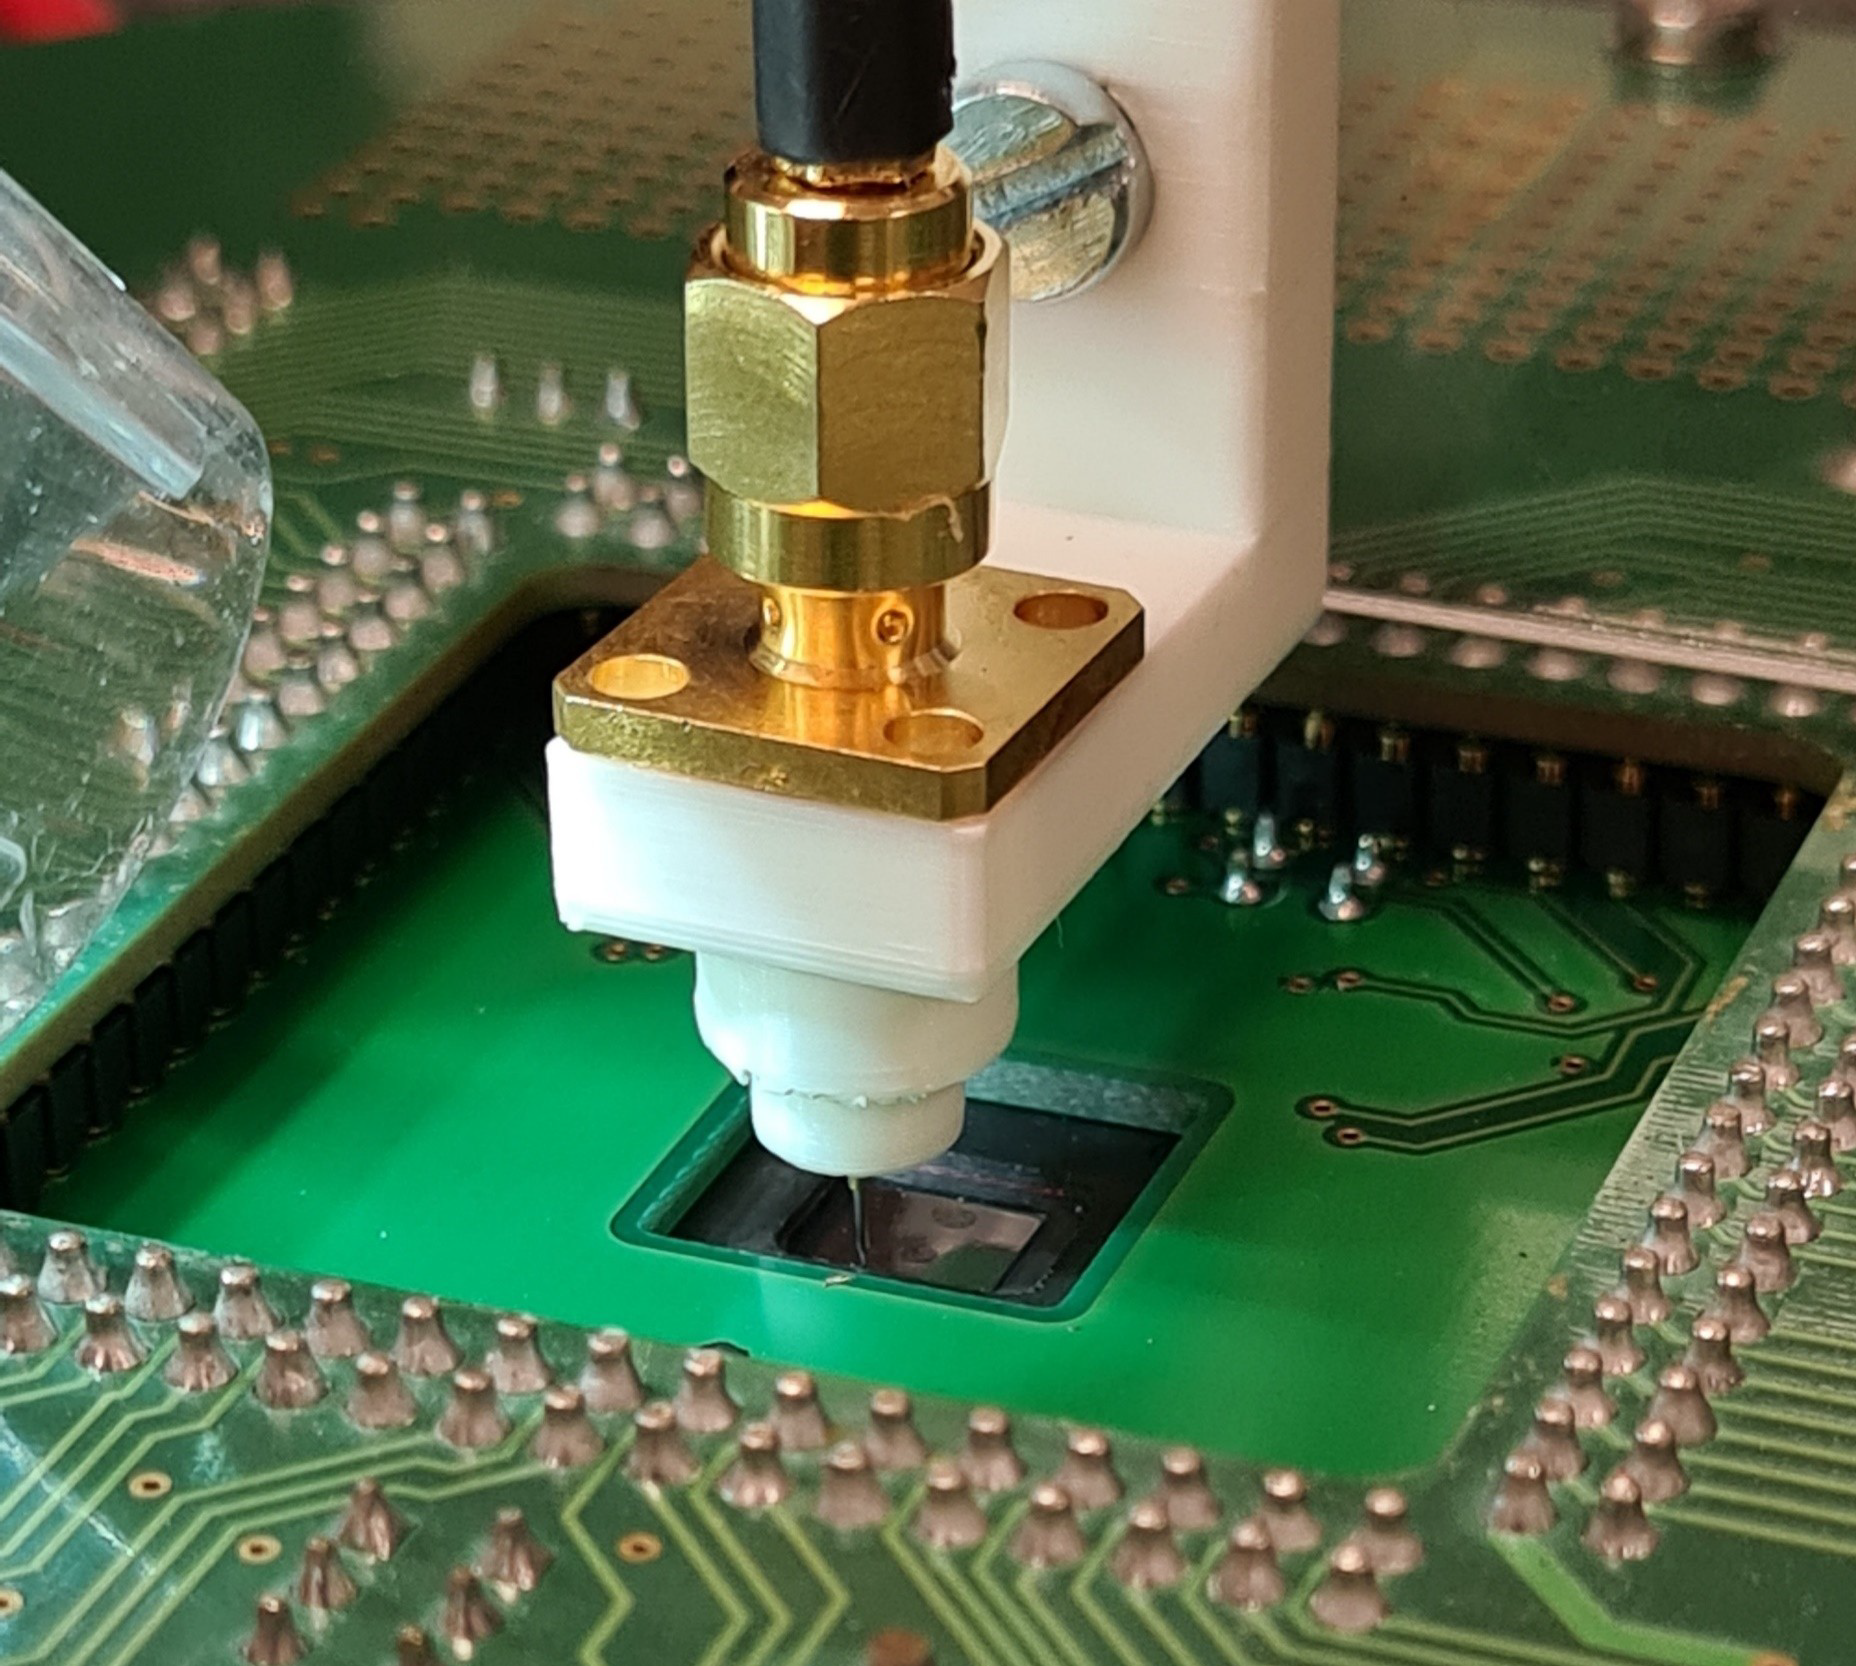
\includegraphics[width=16cm]{2_goodPractices/figures/sondeBBI_loin_raw.png}
%    \caption{BBI metallic probe in mechanical contact with IC target}
%    \label{fig:sondeBBI}
%\end{figure}
%
%\begin{figure}[H]
%    \centering
%    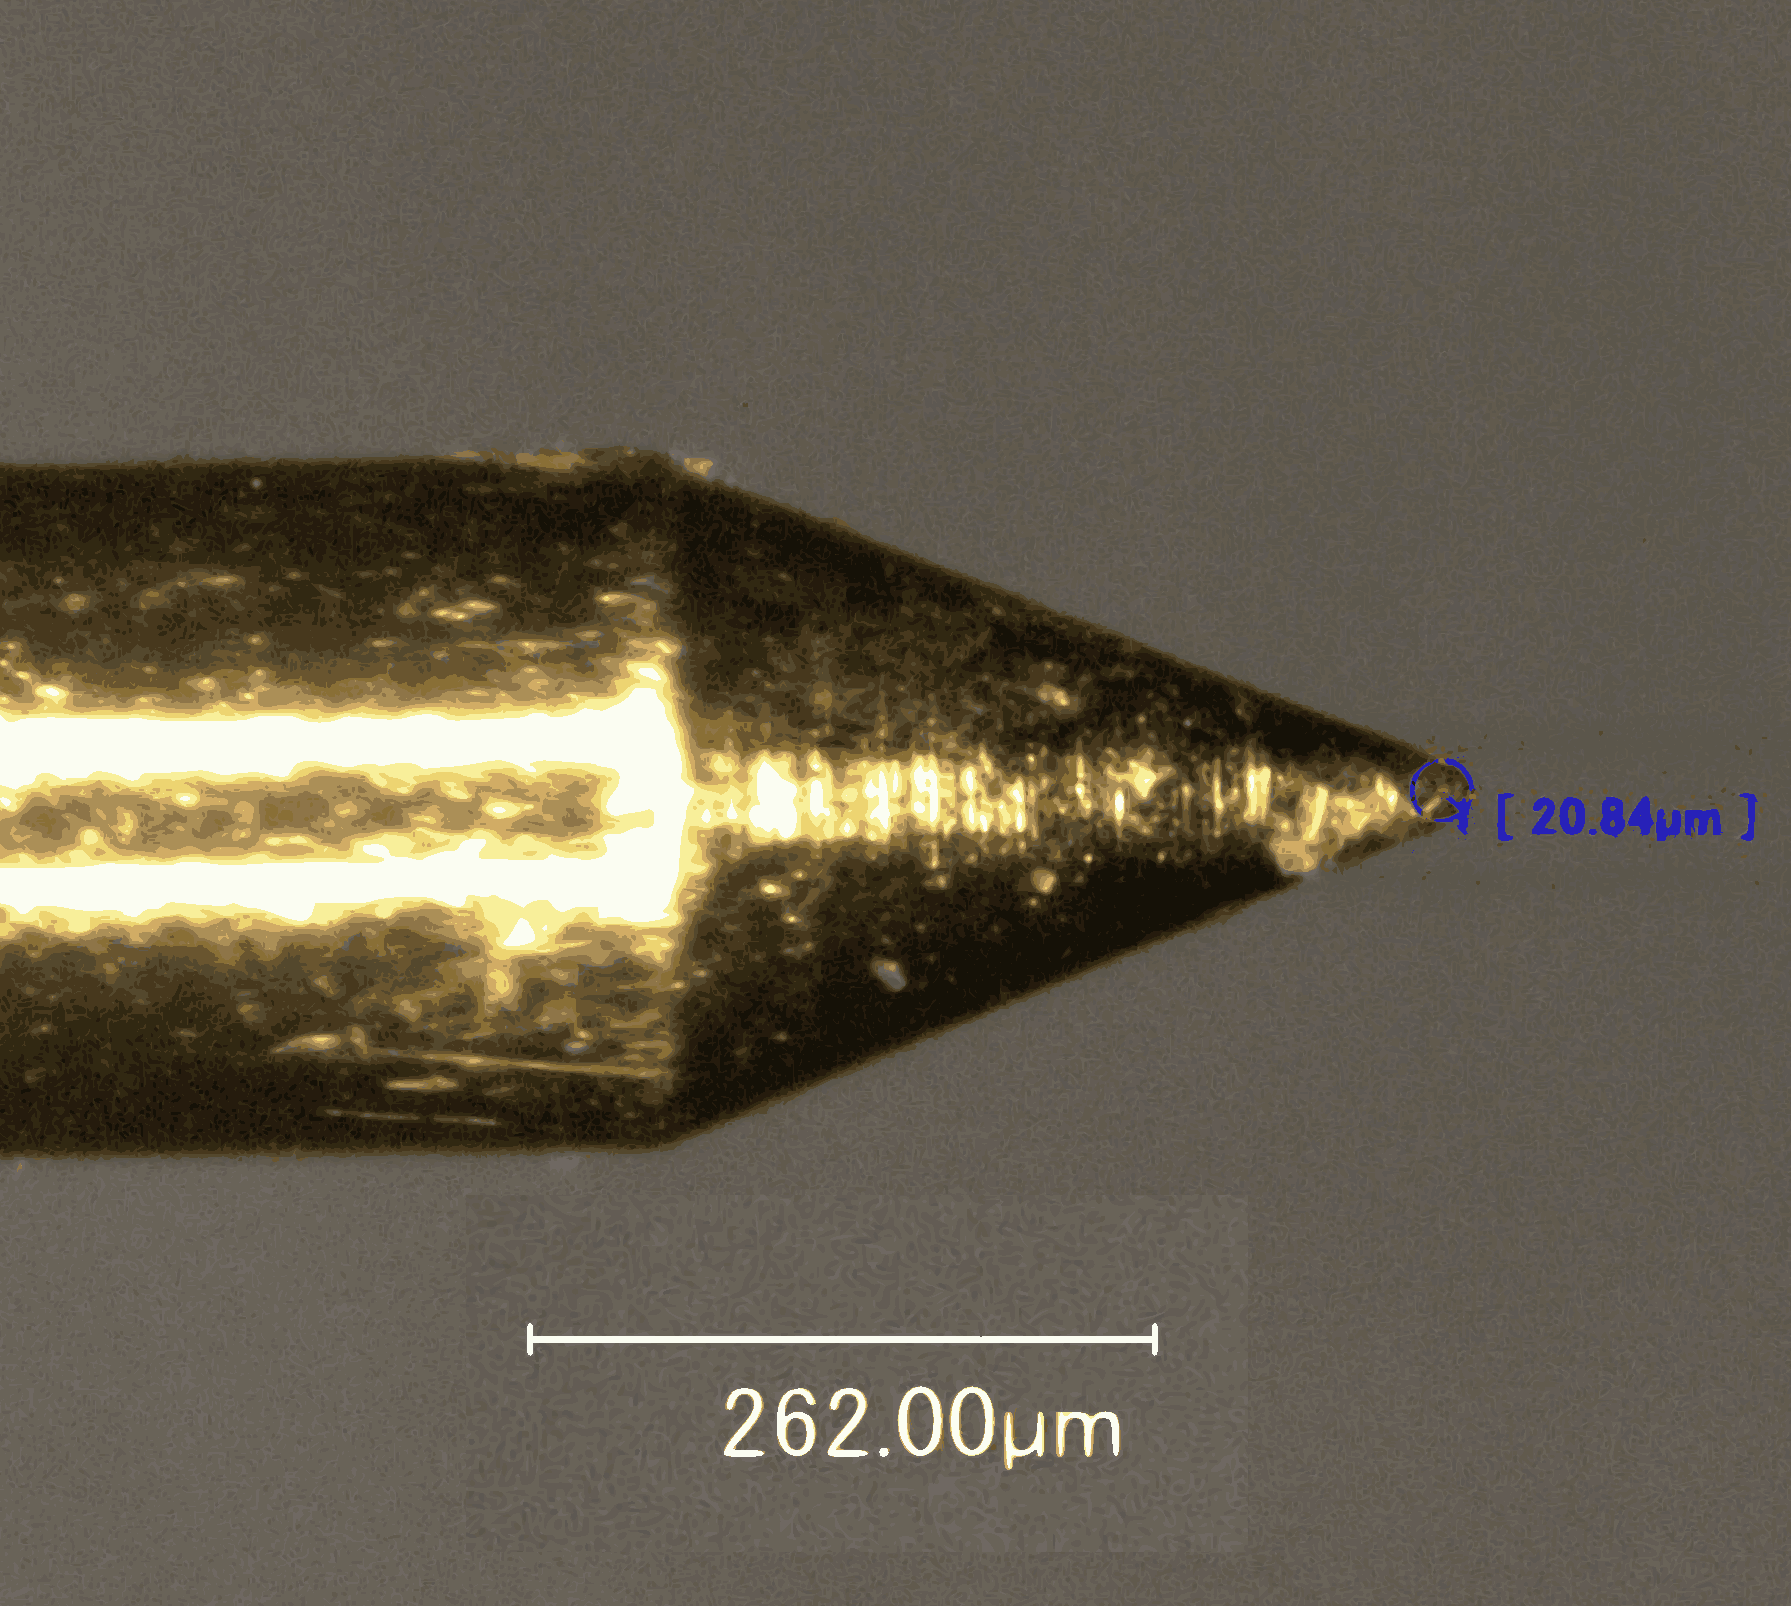
\includegraphics[width=16cm]{2_goodPractices/figures/pointeBBI.pdf}
%    \caption{BBI metallic probe measurement closer look}
%    \label{fig:pointeBBI}
%\end{figure}

\begin{figure}[ht!]
    \centering
    \begin{subfigure}[t]{7.0cm}
        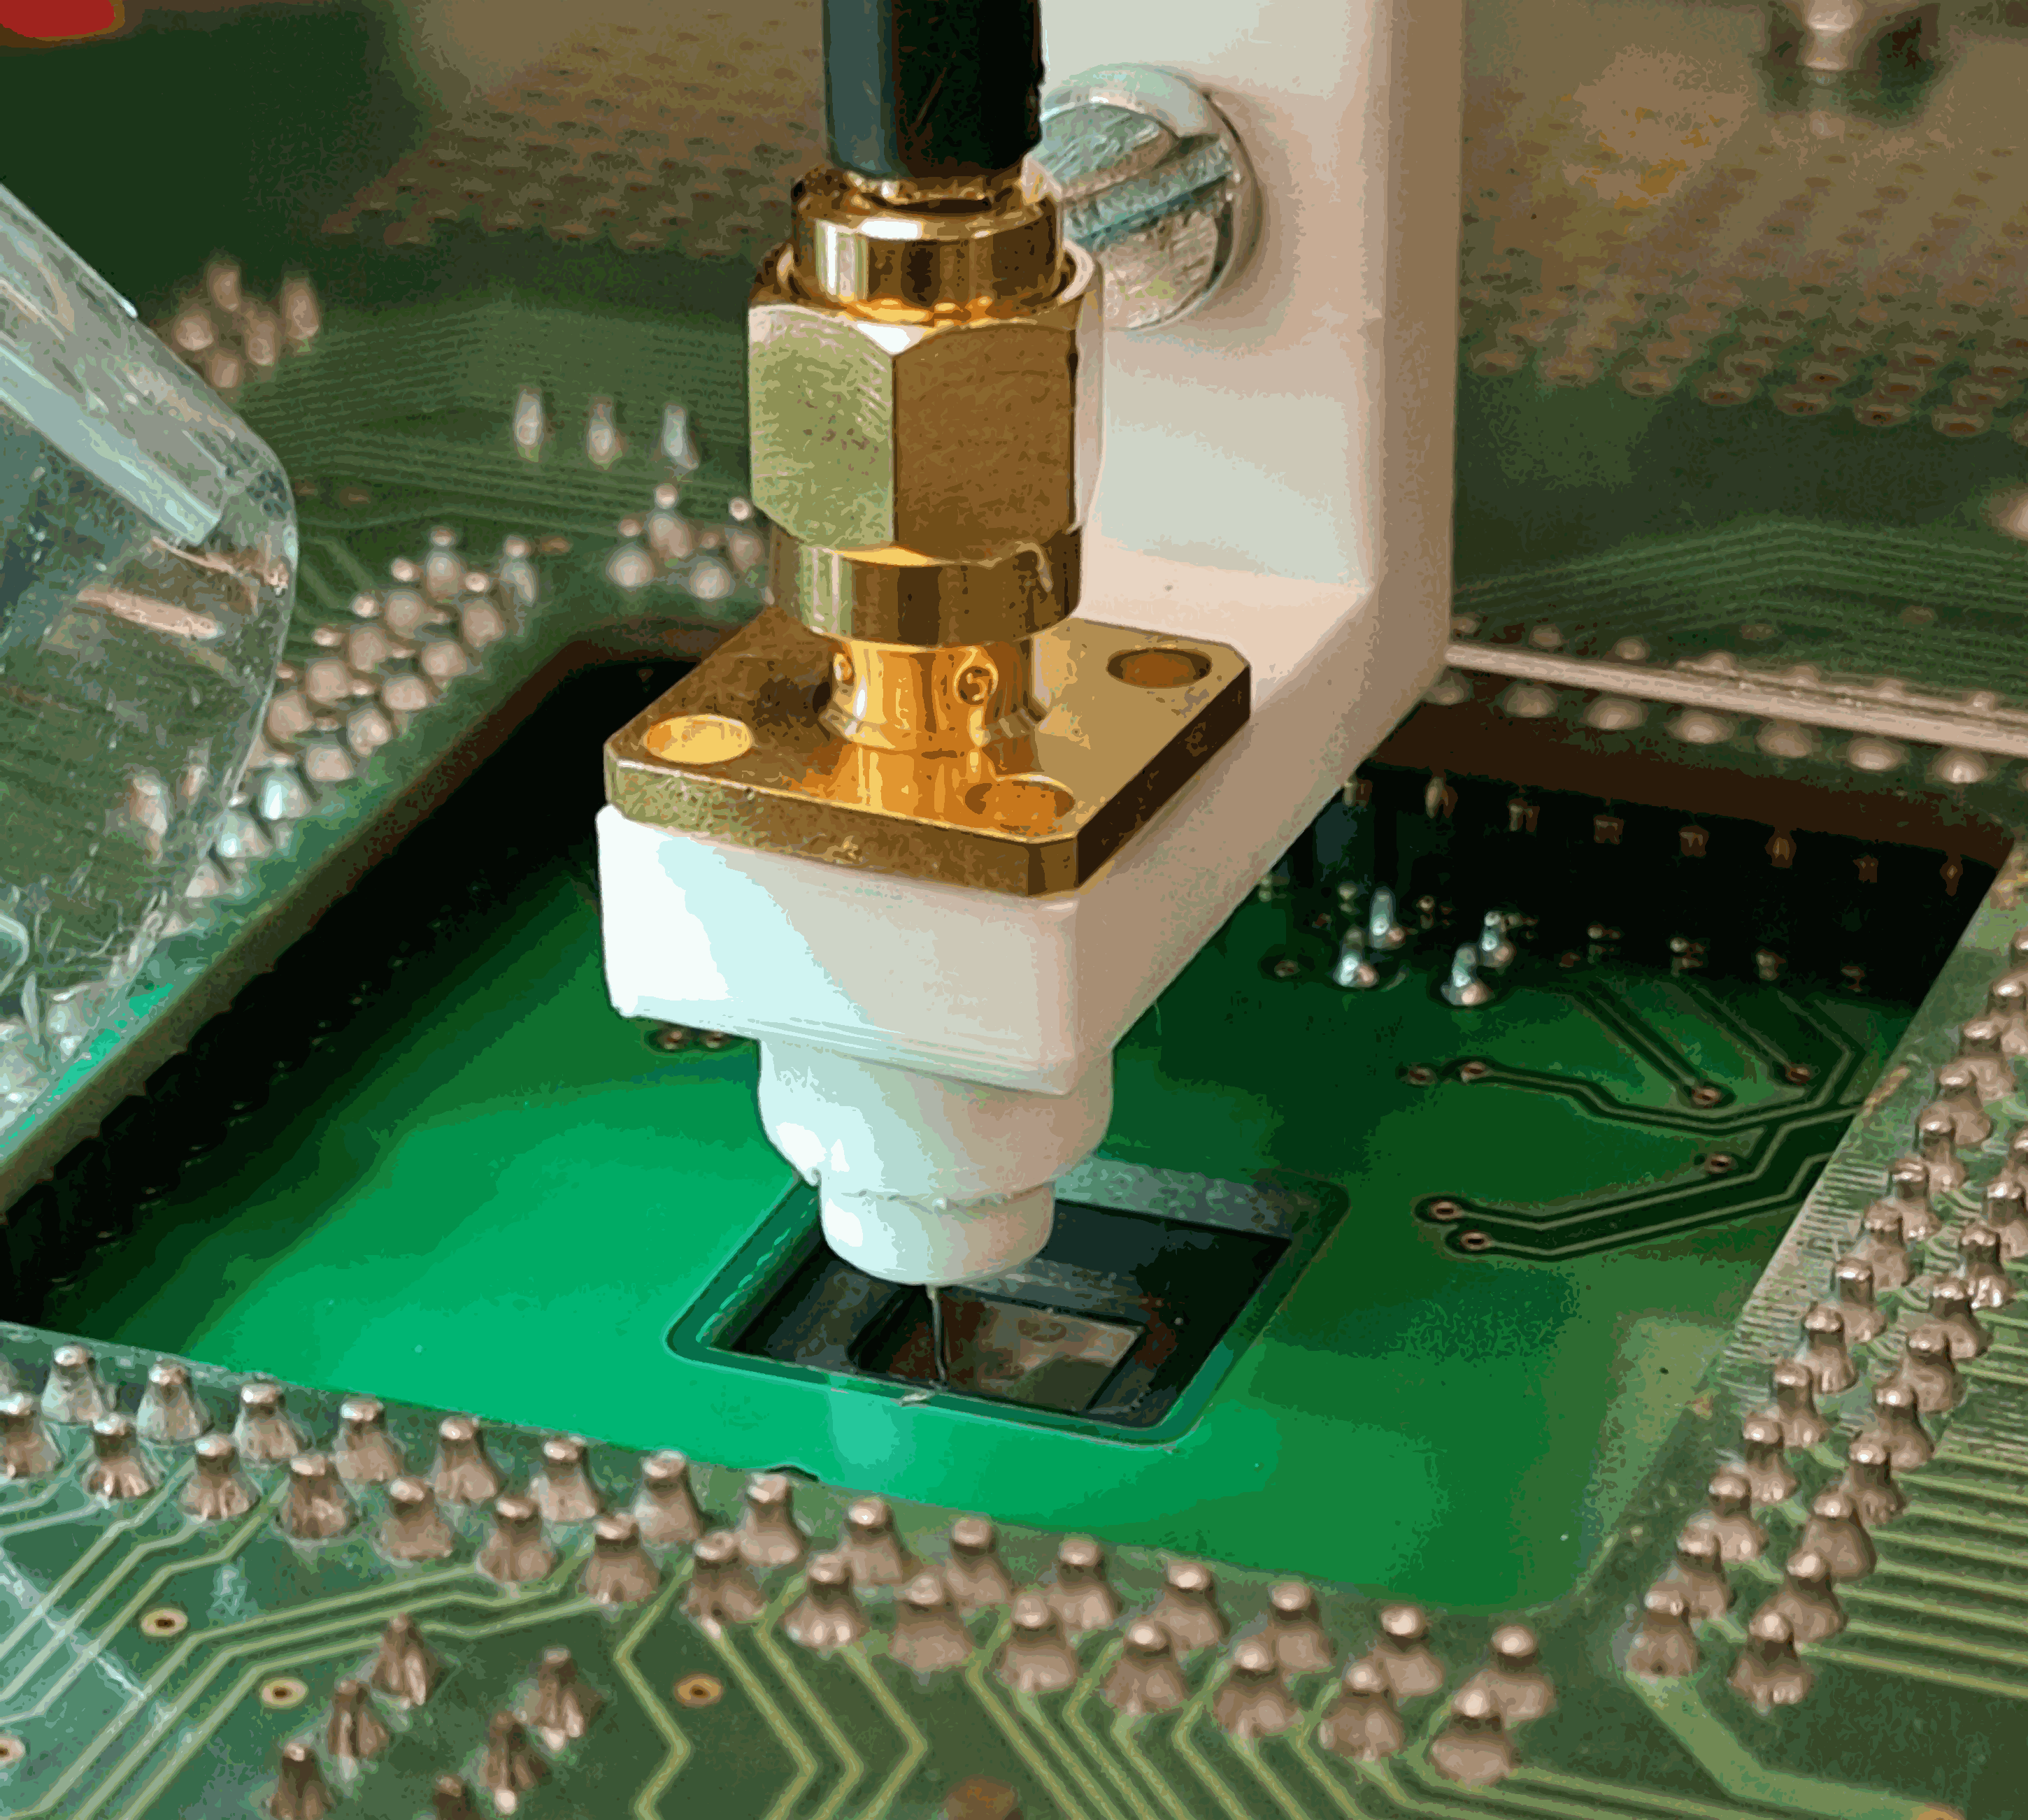
\includegraphics[height=6.8cm]{2_goodPractices/figures/sondeBBI.pdf}
        \caption{BBI metallic probe in mechanical contact with IC target}
        \label{subfig:sondeBBI}
    \end{subfigure}\hfill
    \begin{subfigure}[t]{7.0cm}
        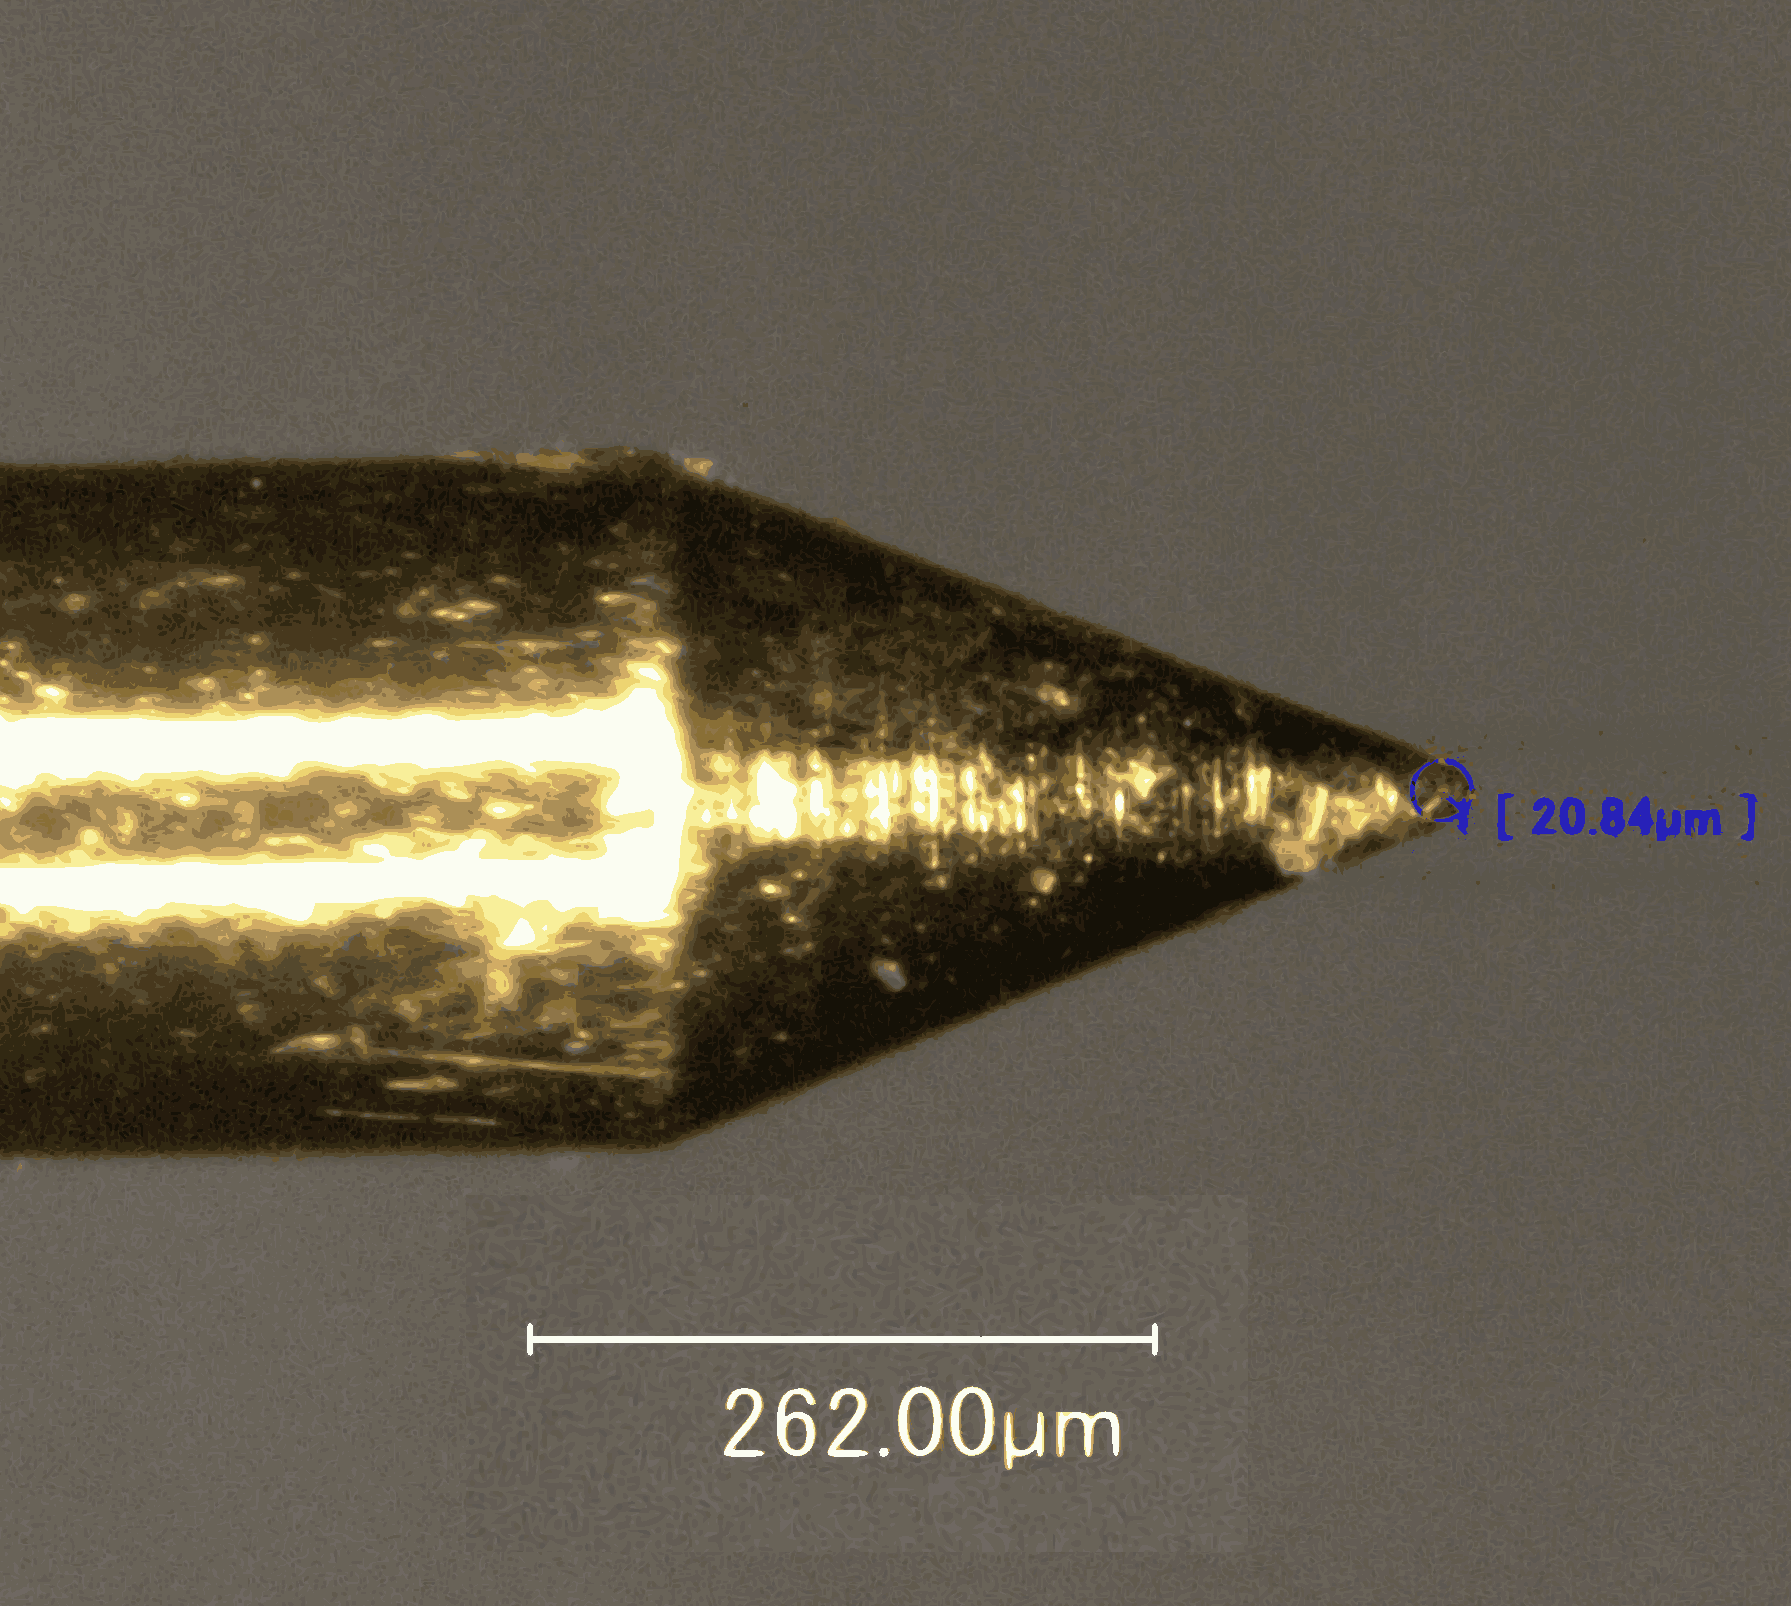
\includegraphics[height=6.8cm]{2_goodPractices/figures/pointeBBI.pdf}
        \caption{BBI metallic probe measurement closer look}
        \label{subfig:pointeBBI}
    \end{subfigure}
    \caption{Dual-well and triple-well inverter silicon sectional view.}
    \label{fig:sondePointeBBI}
\end{figure}

The main piece of equipment when working with BBI is the electrical probe.
It is commonly made with a metal tip, a connector of any sort and a mechanical support to hold everything together.
For the purpose of this work, a custom probe was designed around three simple parts, an SMA connector, in order to have a low-cost, small and standard interconnection, a spring-loaded metallic probe soldered onto the SMA connector, and a custom 3D printed support to hold the structure together.
Fig. \ref{fig:sondePointeBBI} shows detailed pictures of the designed BBI metallic probe, with a global view in operation on Fig.\ref{subfig:sondeBBI}, and a photograph under a microscope of the probe's tip-end on Fig. \ref{subfig:pointeBBI}, allowing to measure its actual size before the first usage.
The metallic probe used has a 0.635 mm diameter and is 16.35 mm long. The specified maximum nominal current of the probe is of 1.5 A, and the electrical contact resistance measures 70 m\textOmega.


\begin{figure}[H]
    \centering
    \includegraphics[width=\textwidth]{2_goodPractices/figures/picoemp-red.jpeg}
    \caption{ChipSHOUTER\textregistered-PicoEMP from NewAE Technology Inc.}
    \label{fig:newAeChipShouter}
\end{figure}
Another fundamental piece of equipment for the practice of BBI is the voltage pulse generator.
It is, generally, the most expensive hardware tool required.
However, nowadays, cheap solutions are easily available, like the NewAE Technology Inc. ChipSHOUTER\textregistered-PicoEMP for example, illustrated in Fig. \ref{fig:newAeChipShouter}.
In addition to being cheaper than most industrial solutions, its design sources are available online, making it a future-proof solution.
In contrast to more expensive solutions, it has inevitably some drawbacks:
\begin{itemize}
    \item The output transformer is low-power, around up to 200 mW
    \item Its recovery time is slow, from 1 to 4 seconds between pulses
    \item It can generate maximum voltage pulses of approximately 250 V
    \item There is no pre-calibration
    \item The pulse width control is not as reliable as other solutions
\end{itemize}
%Nonetheless, during this work, the generator used is the AVTECH AVRK-4-B, which a high speed, precise, voltage pulse generator.
%It allows generating positive or negative pulses up to 750 V of amplitude with a 4 ns rise or fall time, with pulse widths ranging from 6 ns to 20 ns.
%It allowed us to finely tune each setting in order to perform reproducible experiments.
%
%Another very important piece of equipment used for BBI is the probe.
%It simply consists in a metallic tip soldered to an SMA connector.
%However,